\documentclass[11pt,a4paper,twoside,french,svgnames]{report}
\usepackage[utf8]{inputenc} % force the use of utf8
\usepackage[T1]{fontenc} % font encoding, allows accents (T1 font encoding is an 8-bit encoding)
\usepackage[top=2.5cm,bottom=2.5cm,outer=2.5cm,inner=2.5cm]{geometry} % http://tex.stackexchange.com/questions/62311/a4paper-where-should-i-declare-it-in-document-class-or-geometry // another option: papersize={21cm,29.7cm}
\usepackage[french]{babel} % translate everything in the desired language: table of contents, etc. 'english' can be replaced with 'francais'
\usepackage[toc,page,header]{appendix} % cool appendices
\usepackage{graphicx} % images management
\usepackage{wrapfig} % floating images
\usepackage[format=plain,labelfont=bf,font=small,justification=centering,margin=10pt]{caption} % allow multiline captions in figures,
\usepackage{float} % allow \begin{figure}[H] and \begin{table}[H] (to really force positionning, unlike h!)
\usepackage{array} % allow arrays
\usepackage[super]{nth} % allow to write \nth(1) to write 1st, etc
\usepackage{fancyhdr} % headers/footers management (overrides empty, plain and headings)
\usepackage{upquote} % without this, lslisting replace vertical singles quotes with curved ones
\usepackage{listings} % code insertion (MUST BE WRITTEN AFTER BABEL)
\usepackage[
            backend=biber,
            style=numeric,
            sorting=none, % nty = name title year
            url=true, % always show url when provided
            ]{biblatex}
%\usepackage{pdfpages} % include PDF documents
\usepackage{enumitem} % for /setlist
\usepackage{color,soul} % add some colors and hightlight
\usepackage{xcolor} % more colors
\usepackage{afterpage} % allow to execute command after the current page ends
\usepackage[hidelinks,
            colorlinks  = false, % no borders, colors enabled
            anchorcolor = blue,
            linkcolor   = black, % links in table of contents
            urlcolor    = blue,
            citecolor   = blue,
            breaklinks  = true]{hyperref}
\newcommand{\MYhref}[3][blue]{\href{#2}{\color{#1}{#3}}}%

% List settings
\setlist{itemsep=.5em}
\setlist[itemize,2]{label={$\bullet$}} % use bullets for nested itemize in level 2

% REQUIRE
% \usepackage{color}
% \usepackage{listings} % (MUST BE WRITTEN AFTER BABEL)

% General colors
\definecolor{comment}{rgb}{0.12, 0.38, 0.18 } % adjusted, in Eclipse: {0.25, 0.42, 0.30 } = #3F6A4D
\definecolor{keyword}{rgb}{0.2, 0.2, 0.8}
\definecolor{string}{rgb}{0.06, 0.10, 0.98} % #101AF9

% Language-specific colors
% JavaScript
\definecolor{darkgray}{rgb}{.4,.4,.4}
%\definecolor{purple}{rgb}{0.65, 0.12, 0.82}

% hack to force UTF-8 compatibility (for french only)
\lstset{
       extendedchars=true,
       literate={à}{{\`a}}1 {â}{{\^a}}1 %                         lettre a
                {À}{{\`A}}1 {Â}{{\^A}}1 %                         lettre A
                {ç}{{\c{c}}}1 %                                   lettre c
                {Ç}{{\c{C}}}1 %                                   lettre C
                {é}{{\'e}}1 {è}{{\`e}}1 {ê}{{\^e}}1 {ë}{{\"e}}1 % lettre e
                {É}{{\'E}}1 {È}{{\`E}}1 {Ê}{{\^E}}1 {Ë}{{\"E}}1 % lettre E
                {î}{{\^i}}1 {ï}{{\"i}}1 %                         lettre i
                {Î}{{\^I}}1 {Ï}{{\"I}}1 %                         lettre I
                {ô}{{\^o}}1 %                                     lettre o
                {Ô}{{\^O}}1 %                                     lettre O
                {œ}{{\oe}}1 %                                     lettre oe
                {Œ}{{\OE}}1 %                                     lettre OE
                {ù}{{\`u}}1 {û}{{\^u}}1 {ü}{{\"u}}1 %             lettre u
                {Ù}{{\`U}}1 {Û}{{\^U}}1 {Ü}{{\"U}}1 %             lettre U
}

% General rules
\lstset{
  rulecolor=\color{black!50},
  backgroundcolor = \color{blue!10},
  numbers=none, %left % display line numbers
  showspaces=false,
  showtabs=false,
  breaklines=true,
  showstringspaces=false,
  breakatwhitespace=false,
  commentstyle=\color{comment},
  keywordstyle=\color{keyword},
  stringstyle=\color{string},
  basicstyle=\ttfamily,
  extendedchars=true,
  emph=[2]{In},
  emphstyle=[2]\color{black!70},
  morecomment=[l][\color{blue}]{Out},
  frame=single,
  frameround=tttt,
  framerule=0.3pt,
  framesep=4pt,
  belowcaptionskip=2.1pt
}

% % Define "Javascript" because lstlistings doesn't know it
% Taken from https://gist.github.com/Geruhn/3d21f60a869457373d84
\lstdefinelanguage{javascript}{
  keywords={break, case, catch, continue, debugger, default, delete, do, else, false, finally, for, function, if, in, instanceof, new, null, return, switch, this, throw, true, try, typeof, var, void, while, with},
  morecomment=[l]{//},
  morecomment=[s]{/*}{*/},
  morestring=[b]',
  morestring=[b]",
  ndkeywords={class, export, boolean, throw, implements, import, this},
  %keywordstyle=\color{blue}\bfseries,
  ndkeywordstyle=\color{darkgray}\bfseries,
  identifierstyle=\color{black},
  %commentstyle=\color{purple}\ttfamily,
  %stringstyle=\color{red}\ttfamily,
  sensitive=true
}

% Usage: \javascript
\newcommand{\javascript}{\lstset{
  language=javascript,
  title={{\setlength{\fboxsep}{1pt}\fcolorbox{orange}{yellow!20}{\sffamily\scriptsize
              \textcolor{gray!10}{\_}JavaScript\textcolor{gray!10}{\_}}}}
  }
}

% Usage: \code{My title}
\newcommand{\code}[1]{\lstset{
  language=,
  title={{\setlength{\fboxsep}{1pt}\fcolorbox{orange}{yellow!20}{\sffamily\scriptsize
              \textcolor{gray!10}{\_}{#1}\textcolor{gray!10}{\_}}}}
  }
}

% Usage: \sql
\newcommand{\sql}{\lstset{
  language=SQL,
  title={{\setlength{\fboxsep}{1pt}\fcolorbox{orange}{yellow!20}{\sffamily\scriptsize
              \textcolor{gray!10}{\_}SQL\textcolor{gray!10}{\_}}}}
  }
}

% Usage: \fakeshell
\newcommand{\fakeshell}{\lstset{
  language=bash
  }
}

\newcommand{\perl}{\lstset{
  language=perl
  }
}

\newcommand{\xml}{\lstset{
  language=xml
  }
}

% REQUIRES
% Nothing

% Redefine chapter titles: only display the title and remove useless blank space
% Original "/usr/share/texlive/texmf-dist/tex/latex/base/report.cls" edited
\makeatletter
  \def\@makechapterhead#1{% chapter{}
  \vspace*{0\p@}% 50 before
  {\parindent \z@ \raggedright \normalfont
    %\ifnum \c@secnumdepth >\m@ne
    %    \huge\bfseries \@chapapp\space \thechapter
    %    \par\nobreak
    %    \vskip 20\p@
    %\fi
    \interlinepenalty\@M
    \Huge \bfseries \thechapter\quad #1   
    \vskip 40\p@
  }}
  \def\@makeschapterhead#1{% chapter*{}
  \vspace*{0\p@}% 50 before
  {\parindent \z@ \raggedright
    \normalfont
    \interlinepenalty\@M
    \Huge \bfseries  #1\par\nobreak
    \vskip 40\p@
  }}
\makeatother
% REQUIRES
% \usepackage{fancyhdr} % headers/footers management (overrides empty, plain and headings)

% THE ORDER IS REALLY IMPORTANT, OTHERWISE IT WILL BREAK THINGS

% 1.
% Redefines the existing 'plain' style, (because 'chapter' and \tableofcontents ignores the page style currently in effect for their first page)
\fancypagestyle{plain}{
    % Took from: http://anorien.csc.warwick.ac.uk/mirrors/CTAN/macros/latex/contrib/fancyhdr/fancyhdr.pdf
    \fancyhead[LO,RE]{\slshape \leftmark}
    \fancyhead[LE,RO]{\slshape \rightmark}

    % Footers
    \renewcommand{\footrulewidth}{0.4pt}
    \fancyfoot[C]{Rapport de TD -- Steve \textsc{Lagache} \& Romain \textsc{Pellerin}}
    \fancyfoot[LE,RO]{\ifdefined\thepage \thepage \fi} % to be used with \pagenumbering{gobble} % no numerotation
    % \fancyfoot[LE,RO]{\ifnum\thepage>0 \thepage \fi} % to be used with %\addtocounter{page}{-4} % numerotation begins at 1 + (-4)
}

% 2.
\pagestyle{plain}

% 3.
% http://tex.stackexchange.com/questions/111223/markboth-is-not-working-when-using-chapter-and-section
% Took from : http://ftp.snt.utwente.nl/pub/software/tex/macros/latex/contrib/fancyhdr/fancyhdr.pdf
\renewcommand{\chaptermark}[1]{\markboth{}{\MakeUppercase{\thechapter.\ #1}}}
\renewcommand{\sectionmark}[1]{}

% NORMALLY
% \renewcommand{\chaptermark}[1]{\markboth{\MakeUppercase{\thechapter.\ #1}}{}}
% \renewcommand{\sectionmark}[1]{\markright{\thesection.\ #1}}
 % To be edited to change the header and footer

\title{Rapport de TD}
\author{Steve LAGACHE et Romain PELLERIN}
\date\today
\setcounter{tocdepth}{2} % ToC depth

\pagenumbering{arabic} % re-enable numering

\begin{document}
\thispagestyle{empty} % only applies to this page
\begin{center}

\includegraphics[height=3cm]{images/logo-utc.png}

\vspace{4cm}

\noindent{\LARGE\MYhref[black]{http://www.utc.fr/}{Université de Technologie de Compiègne}}

\vspace{1cm}

{\large Génie Informatique}

\vspace{3cm}
\noindent\fbox{
\begin{minipage}{.9\textwidth}
\begin{center}
    \vspace{0.3cm}\Large{Rapport de TD}\\
    \vspace{0.3cm}\LARGE{\textbf{LO17}}\vspace{0.3cm}\\
\end{center}
\end{minipage}}

\vspace{3cm}

\begin{tabular}{>{\hfill\arraybackslash}p{5cm}p{5cm}}
%\hline
    \multicolumn{2}{c}{\textbf{Steve \textsc{LAGACHE} \& Romain \textsc{PELLERIN}}}\\\\
%\hline
    \multicolumn{2}{c}{Chargé de TD : Pierre \textsc{Morizet-Mahoudeaux}}\\\\
%\hline
    \multicolumn{2}{c}{Printemps 2016 (P16)}\\
%\hline

\end{tabular}
\vfill

{\footnotesize Dernière mise à jour: \today}
\end{center}


\tableofcontents

\chapter{TD1: Génération XM}

L'objectif de ce TD était de s'initier au ``\textit{parsing}'' en Perl et d'être capable d'extraire certaines informations (uniques ou non) d'un seul document d'abord, puis ensuite de plusieurs. Nous avions un peu plus de 300 pages HTML contenant toute un article issu d'un même site scientifique. Il nous fallait extraire des données ``uniques'' comme le numéro de l'article ou sa rubrique, et des données présentes une (parfois zéro) ou plusieurs fois, comme les paragraphes du texte principal ou les images présentes.

\section{Méthodologie employée}

Pour la totalité des éléments à récupérer, nous avons utilisé des \textit{regex} (sauf pour le nom du fichier que nous récupérerions dans \lstinline{$ARGV}).

Pour produire notre XML, nous avons décidé de tout afficher sur la sortie standard. Il s'agira ensuite de rédiriger cette sortie standard dans un fichier grâce à l'opérateur \lstinline{>} d'Unix.

\subsection{Repérer un élémént d'intérêt}

Pour chaque élément unique qu'il nous fallait récupérer, nous avons essayer de trouver la structure de balises HTML avoisinante qui soit unique. Pour cela, nous avons beaucoup fait appel à la structure \lstinline{.*?} (n'importe quel caractère zéro, une ou plusieurs fois) dans son mode \textit{lazy}. Cela nous a permis de simplifier nos \textit{regex}.\\
Voyons quelques exemples. Pour récupérer le numéro, la structure HTML autour était suffisamment simple pour ne pas utiliser ``n'importe quel caractère'' :

\perl
\begin{lstlisting}
$body=~/<span class="style95" style="color:inherit">(\d+)<\/span><\/a>/;
\end{lstlisting}

En revanche, nous en avons eu besoin pour la partie contact :

\begin{lstlisting}
$body =~ /Pour en savoir plus, contacts :.*?<p class="style44"><span class="style85">(.*?)<\/span>/s;
\end{lstlisting}

\subsection{Lecture du contenu d'un fichier}

Nous avons été capables de récupérer le contenu d'un fichier donné en argument grâce à une boucle sur l'opérateur ``diamant'' (\lstinline{<>}). Fondalement, cet opérateur permet de boucler sur chaque ligne de l'\textit{input}. Nous avons donc simplement récupéré chaque ligne du fichier et avons concaténé ces lignes à une variable \lstinline{$body} initialisée à une chaîne de caractères vide.

\subsection{Lecture du contenu de plusieurs fichiers}

Pour pouvoir récupérer toutes les lignes de chaque fichier tout en dissociant les fichiers, nous avons du opter pour une technique légèrement différente.

\begin{enumerate}
  \item Nous créons une tableau.
  \item Chaque ``case'' du tableau sera une variable similaire à \lstinline{$body} (dont nous avons parlé au-dessus): elle contiendra toutes les lignes \textbf{d'un seul fichier}.
  \item Grâce à l'opérateur diamant, nous bouclons sur toutes les lignes de l'\textit{input}.
  \item Nous sommes capable de savoir à tout instant quel fichier nous sommes en train de lire grâce à la variable \lstinline{$ARGV}.
  \item Une fois que nous avons récupéré tous les différents documents dans chaque case du tableau, nous commençons à boucler sur ce tableau de la même manière que nous le faisions pour un seul fichier.
\end{enumerate}

\perl
\begin{lstlisting}
@htmls;
while (<>) {
  $fichier = $ARGV;
  $fichier=~s/.*\///g;
  if (!defined(@htmls{$fichier})) {
    $htmls{$fichier} = $_;
  }
  else {
    $htmls{$fichier} .= $_;
  }
}

print "<corpus>\n";
while (($fichier,$html) = each(%htmls)) {
  print "<bulletin>\n";
  ...
  print "</bulletin>\n";
  }
print "</corpus>\n";
\end{lstlisting}

À noter que nous n'avons pas utilisé la fonction \lstinline{chop} pour les lignes de l'\textit{input}. Cela n'a pas beaucoup d'incidence, il nous faudra seulement penser dans nos futurs regex à prendre en compte le caractère \lstinline{\n} (souvent en utilisant l'option \lstinline{/s}).

\section{Commandes Unix}

\subsection{Génération du XML}
\fakeshell

Voici la commande Unix utilisée pour récupérer la sortie standard de notre programme et la rediriger dans un fichier XML. Il faut également préciser que nous avons rendu notre programme exécutable grâce à \lstinline{chmod}. De plus, nous utilisons le script \lstinline{convert.pl} pour convertir les entités HTML en caractère Unicode.

\begin{lstlisting}
./td1.pl BULLETINS/*.htm | perl convert.pl > output.xml
\end{lstlisting}

\subsection{Vérification du nombre d'images}

Nous avons également utilisé quelques commandes Unix supplémentaires dans le but de vérifier que nous récupérerions bien le nombre exactes d'images présentes dans les articles. Par exemple, nous avons utilisé \lstinline{grep} dans son mode \textit{regex}.

\begin{lstlisting}
./td1.pl BULLETINS/*.htm | perl convert.pl > output.xml && { grep "<image>" output.xml } | wc -l && echo "Images parsées en Perl" && { grep -aoE "streaming.+?\.jpg" BULLETINS/*.htm && grep -aoE "<img.*?www\.bulletins-electroniques\.com\/Resources_fm\/actualites.*?\.jpg" BULLETINS/*.htm } | wc -l && echo "Images dans les fichiers d'origine";
\end{lstlisting}

\begin{figure}[H]
  \centering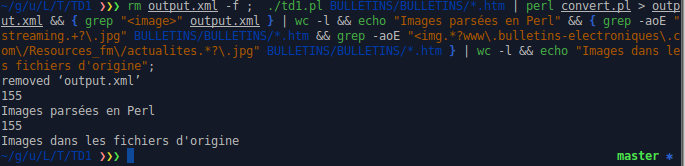
\includegraphics[width=1.00\textwidth]{images/output_td1.png}
  \caption{Résultat de la commande}
\end{figure}

Ce n'est cependant pas la meilleure technique puisque nous réutilisons les mêmes \textit{regex} que celles utilisées dans notre script Perl.\\
Une meilleure solution consisterait à compter toutes les balises image dans les fichiers et à soustraire le nombre d'images qui ne font pas partie des articles (celles sur les côtés par exemple).
% pour l'index, parler de la granularité (bulletin, article) (question 1.1)

\chapter{TD2: Indexation}

Le but de ce second TD est d'utiliser le fichier XML que nous avons produit lors du TD1 afin de créer des index (des fichiers inverses). Pour cela, nous avons à notre disposition plusieurs scripts Perl.

\begin{enumerate}
  \item \textbf{segmente\_TT.pl}: permet, à partir d'un fichier XML, d'extraire tous les mots individuellement contenus entre les balises \lstinline{<titre>} ou \lstinline{<texte>}.
  \item \textbf{newcreeFiltre.pl}: permet de créer un script Perl à partir d'un fichier à une ou deux colonnes : ce script généré remplacera les mots de la première colonne par ceux de la seconde (ou par rien s'il n'y a qu'une colonne) dans un fichier donné en paramètre à ce script.
  \item \textbf{successeurs.pl} et \textbf{filtronc.pl} ; ces deux scripts s'utilisent de pair, afin de :
  \begin{enumerate}
    \item Générer la liste des succésseurs pour chaque lettre des mots d'une liste de mots.
    \item Créer à partir des résultats obtenus à un fichier à deux colonnes associant un mot à un lemme.
  \end{enumerate}
  \item \textbf{index.pl}: permet de créer à partir d'un corpus (XML) un fichier inverse sur une balise donnée en argument
  \item \textbf{indexText.pl} ; permet de créer un fichier inverse à partir d'un flux de données (entrée standard) de la forme ``mot rubrique fichier numéro''.
\end{enumerate}

\section{Obtenir les tf}
\fakeshell

Grâce au premier script, nous sommes capable d'obtenir la liste des mots contenus dans les textes et titres de tous les documents HTML. Puis, à l'aide des commandes Unix telles que \lstinline{sort} et \lstinline{uniq} (avec l'argument \lstinline{-c}), nous obtenons pour chaque mot son \textbf{tf} (nombre d'occurences).

\begin{lstlisting}
cat ../TD1/output.xml| ./segmente_TT.pl -f | sort | uniq -c | sed -e 's/^\s*//' > tf.txt
\end{lstlisting}

La commande \lstinline{sed} nous permet de supprimer les espaces inutiles en début de chaîne, qui sont automatiquement générés par les commandes.

\section{Obtenir les df}

Ensuite, pour obtenir les \textbf{idf} (nombre de fichiers dans lesquel un mot apparaît), nous avons deux possibilités: réutiliser le fichier \textbf{tf.txt} directement ou repartir du fichier XML produit lors du TD1. Voici comment faire à partir du fichier \textbf{tf.txt}:

\begin{lstlisting}
cat tf.txt | cut -d' ' -f2 | cut -f1 | sort | uniq -c | sed -e 's/^\s*//' > df.txt
\end{lstlisting}

Ici à nouveau nous retirons les espaces en début de chaine. La commande \lstinline{cut} nous permet de sélectionner uniquement certaines ``colonnes'' de notre fichier source.

\section{idf}

Ensuite, nous devons calculer les \textbf{idf} des mots. Cela implique notamment de calculer un logarithme 10. Nous avons donc créer un script Perl qui prend en argument notre fichier texte contenant les df. Le sortie standard de ce script est redirigée vers un fichier \lstinline{idf.txt}.

\perl
\begin{lstlisting}
sub log10 {
    my $n = shift;
    return log($n)/log(10);
}

while (<>) {
    /(\d+)\s+(.*)/;
    print $2."\t".log10(326/$1)."\n";
}
\end{lstlisting}

\section{tf*idf}

La dernière étape avant de passer aux stop-lists est de caculer le quotient \textbf{tf*idf}. Cela se fait très facilement grâce à un script Perl utilisant un tableau associatif. Le script traite d'abord un fichier texte contenant les idf, en les stockant dans ce tableau. Ensuite, le script traire le fichier concernant les tf: c'est la que la multiplication est faite et que le résultat est affiché sur la sortie standard (que l'on va bien sûr rediriger vers un fichier).

\begin{lstlisting}
# Usage: perl % idf.txt tf.txt

@mots;
while (<>) {
    if ($ARGV =~ m/idf/) {
        /(.*?)\s+(\d+(\.\d+)?)/;
        $mots{$1} = $2;
    }
    elsif ($ARGV =~ m/tf/) {
        /(\d+)\s+(.*?)\s+(.*)/;
        $nb = $1;
        $mot = $2;
        $file = $3;
        $tfidf = $nb * ($mots{$mot});
        print $file."\t".$mot."\t".$tfidf."\n";
    }
}
\end{lstlisting}
\fakeshell

\section{Lemmes}

Maintenant, il s'agit de générer une stoplist afin de filtrer le fichier XML généré lors du TD1.

\chapter{Conclusion générale}

\section{OpenGL ou Unity}

La plus grosse problématique du projet aura été le choix entre Unity et OpenGL. Nous étions initalement partis sur du développement en OpenGL mais heureusement, en début d'année 2015, Unity a rendu son moteur totalement gratuit, nous permettant ainsi de pouvoir l'utiliser. Nous nous en sommes rendus compte peu de temps après le début du projet et avons ainsi changé de technologie. Nous avons tout de même eu le temps d'essayer OpenGL et il s'était avéré que le développement aurait été bien trop dur et presque impossible. Effectivement, nous ne connaissions pas cette technologie et la contrainte de temps (un semestre) ne nous aurait pas permis de l'appréhender.

\section{Problèmes}

Un autre problème aura été l'utilisation du SDK de Google. Au départ nous ne savions pas comment faire déplacer le joueur, nous étions donc partis sur l'utilisation d'une \textit{library} tierce, Dive. Or il s'est avéré que cette \textit{library} souffrait d'un bug au niveau du gyroscope. Nous avons finalalement réussi à utiliser uniquement le SDK de Google et faire avancer notre joueur.

\section{Jeu final et objectifs}

Au final, un seul de nos objectifs complémentaires a été atteint : rajouter une ambiance sonore (une musique de fond). Nous sommes néanmoins très satisfaits du résultat visuel et du jeu de manière générale. Avoir plus de temps nous aurait probablement permis d'atteindre d'autres objectifs.

\begin{appendices}
\chapter{TD1 : code}

\noindent Ce code fonctionne avec un ou plusieurs fichiers.

\perl

\begin{lstlisting}
#!/usr/bin/perl

use utf8;
binmode(STDOUT, ":utf8");

# HTML AND BODY

@htmls;
while (<>) {
  # FILENAME
  $fichier = $ARGV;
  $fichier=~s/.*\///g;
  s/\n//;
  if (!defined(@htmls{$fichier})) {
    $htmls{$fichier} = $_;
  }
  else {
    $htmls{$fichier} .= $_;
  }
}

print "<corpus>\n";
while (($fichier,$html) = each(%htmls)) {
  print "<bulletin>\n";
  print '<fichier>'.$fichier."</fichier>\n"; # si on donne *.htm en param, argv[0] contient le premier, [1] un autre, etc
  $body = $html;
  $body=~/<body.*?>(.*)<\/body>/sg;
  $body = $1;


  # NUMERO

  $body=~/<span class="style32">BE France (\d+).*?<\/span>/;
  $numero = $1;
  print '<numero>'.$numero."</numero>\n";


  # DATE

  $body=~/<span class="style42">.*?(\d{1,2}\/\d{1,2}\/\d{4})<\/span>/;
  $date = $1;
  print '<date>'.$date."</date>\n";


  # RUBRIQUE AND TITRE

  $body=~/<p class="style96"><span class="style42">(.+)<br><\/span><span class="style17">(.*?)<\/span><\/p>/;
  $rubrique = $1;
  $titre = $2;
  print '<rubrique>'.$rubrique."</rubrique>\n";
  print '<titre>'.$titre."</titre>\n";


  # TEXTE

  $body =~ /<td.*?class="FWExtra2".*?>.*?<span class="style95">(.*?)<td.*?class="FWExtra2"/s;
  $texte = $1;
  $texte =~ s/<br \/>\n?<\/span><div style="text-align: center"><img.*?class="style95"><br \/>//gs;
  $texte =~ s/<.*?>//g;
  $texte =~ s/^\s+|\s+$|\n//g;
  print "<texte>".$texte."</texte>\n";
  # (.*?) makes it lazy (cf http://forums.phpfreaks.com/topic/265751-how-does-it-work/) instead of greedy


  # IMAGES WITH URL

  #@array = ($body =~ /(www\.bulletins-electroniques\.com\/Resources_fm\/actualites.*?\.jpg)/g);
  #print join "--\n", @array;
  print "<images>\n";
  pos($body) = 0; # reset cursor position cause /g leave the cursor in the middle of nowhere
  while ($body =~ /(www\.bulletins-electroniques\.com\/Resources_fm\/actualites.*?\.jpg).*?<strong>(.*?)<\/strong>|(streaming.+?\.jpg)/sg) {
      print "<image>".$1.$3."</image>\n";
      print "<legende>".$2."</legende>\n";
  }
  print "</images>\n";


  # CONTACT

  print "<contact>";
  $body =~ /Pour en savoir plus, contacts :.*?<p class="style44"><span class="style85">(.*?)<\/span>/s;
  $contact = $1;
  $contact =~ s/<.*?>//gs;
  print $contact;
  print "</contact>\n";
  print "</bulletin>\n";

  if (!defined($fichier) || !defined($numero) || !defined($date) || !defined($rubrique) || !defined($titre) || !defined($texte) || !defined($contact)) {
    print STDERR "Missing one field";
    exit -1;
  }
  $fichier = $numero = $date = $rubrique = $titre = $texte = $contact = undef;
}
print "</corpus>\n";
\end{lstlisting}

\end{appendices}

\end{document}
